\documentclass[11pt,letterpaper]{article}

% ============================================================================
% PACKAGES
% ============================================================================
\usepackage[utf8]{inputenc}
\usepackage[T1]{fontenc}
\usepackage{helvet}
\renewcommand{\familydefault}{\sfdefault}
\usepackage[margin=0.85in, headheight=28pt]{geometry}
\usepackage{graphicx}
\usepackage{xcolor}
\usepackage{tikz}
\usepackage{tcolorbox}
\usepackage{booktabs}
\usepackage{enumitem}
\usepackage{hyperref}
\usepackage{fancyhdr}
\usepackage{titlesec}
\usepackage{multicol}
\usepackage{listings}
\usepackage{upquote}
\usepackage{amsmath,amssymb}
\usepackage{array}
\usepackage{longtable}

% Ragged-right paragraph columns to prevent word spacing issues
\newcolumntype{L}[1]{>{\raggedright\arraybackslash}p{#1}}

% Increase vertical spacing between table rows for readability
\renewcommand{\arraystretch}{1.4}

\usepackage{colortbl}
\usepackage{pifont}
\usepackage{setspace}
\usepackage{parskip}
\usepackage{caption}
\usepackage{tabularx}

\usetikzlibrary{shapes.geometric, arrows.meta, positioning, calc, decorations.pathreplacing, backgrounds, fit}

% ============================================================================
% COLOR DEFINITIONS - Laboratory Systems Theme (bioengineering/hardware)
% ============================================================================
% Primary: Forest green - biological, growth, laboratory
\definecolor{labgreen}{HTML}{1B7A3D}
\definecolor{lightteal}{HTML}{20B2AA}
\definecolor{deepforest}{HTML}{0B5345}
% Accent: Instrument gold for highlights and callouts
\definecolor{instrumentgold}{HTML}{B7950B}
\definecolor{safetyamber}{HTML}{F39C12}
% Domain colors
\definecolor{thermalred}{HTML}{C0392B}
\definecolor{fluidblue}{HTML}{2980B9}
\definecolor{visionpurple}{HTML}{7D3C98}
\definecolor{safetygreen}{HTML}{27AE60}
% Neutrals
\definecolor{lightgray}{HTML}{F4F6F7}
\definecolor{medgray}{HTML}{BDC3C7}
\definecolor{softslate}{HTML}{5D6D7E}
\definecolor{textdark}{HTML}{1C2833}

% ============================================================================
% HYPERREF SETUP
% ============================================================================
\hypersetup{
  colorlinks=true,
  linkcolor=deepforest,
  urlcolor=lightteal,
  pdftitle={BioForge: Agent-Driven CRISPR Automation Platform},
  pdfauthor={Hardware Systems Documentation}
}

% ============================================================================
% SPACING AND TYPOGRAPHY
% ============================================================================
\setstretch{1.15}
\setlength{\parskip}{0.5em}
\setlist{nosep, leftmargin=1.5em, itemsep=0.3em}

% ============================================================================
% PAGE STYLE - Laboratory circuit pattern (hardware/bioengineering theme)
% ============================================================================
\pagestyle{fancy}
\fancyhf{}
\fancyhead[L]{%
  \begin{tikzpicture}[baseline=-0.5ex]
    % Circuit-like pattern (hardware/engineering feel)
    \draw[lightteal, opacity=0.5, line width=0.6pt] (0,0.15) -- (0.3,0.15);
    \draw[lightteal, opacity=0.5, line width=0.6pt] (0.3,0.15) -- (0.3,0.3);
    \draw[lightteal, opacity=0.5, line width=0.6pt] (0.3,0.3) -- (0.6,0.3);
    \draw[lightteal, opacity=0.5, line width=0.6pt] (0.6,0.3) -- (0.6,0.0);
    \draw[lightteal, opacity=0.5, line width=0.6pt] (0.6,0.0) -- (0.9,0.0);
    \draw[lightteal, opacity=0.5, line width=0.6pt] (0.9,0.0) -- (0.9,0.15);
    \draw[lightteal, opacity=0.5, line width=0.6pt] (0.9,0.15) -- (1.2,0.15);
    \fill[labgreen, opacity=0.8] (0.3,0.15) circle (0.04);
    \fill[instrumentgold, opacity=0.8] (0.6,0.3) circle (0.04);
    \fill[labgreen, opacity=0.8] (0.9,0.15) circle (0.04);
  \end{tikzpicture}
  \hspace{0.4em}\textcolor{deepforest}{\textsf{\small BIOFORGE-2026-HW-001}}%
}
\fancyhead[R]{\textcolor{softslate}{\textsf{\thepage}}}
\fancyfoot[C]{\textcolor{softslate}{\footnotesize\textsf{Hardware Systems Documentation | Agent-Driven Biological Automation}}}
\renewcommand{\headrulewidth}{0pt}
\renewcommand{\footrulewidth}{0pt}

\fancyheadoffset{0pt}
\setlength{\headheight}{32pt}

% ============================================================================
% SECTION FORMATTING - Laboratory systems style with circuit accents
% ============================================================================
\titleformat{\section}
  {\normalfont\LARGE\bfseries\color{deepforest}}
  {\thesection}{0.8em}{}[\vspace{-0.3em}{\color{lightteal}\rule{\textwidth}{1.5pt}\hspace{-\textwidth}\color{labgreen}\rule{3cm}{1.5pt}}]
\titleformat{\subsection}
  {\normalfont\Large\bfseries\color{deepforest}}
  {\thesubsection}{0.6em}{}
\titleformat{\subsubsection}
  {\normalfont\large\color{softslate}\bfseries}
  {\thesubsubsection}{0.5em}{}

\titlespacing*{\section}{0pt}{3ex plus 1ex minus .2ex}{2ex plus .2ex}
\titlespacing*{\subsection}{0pt}{2.5ex plus 1ex minus .2ex}{1.5ex plus .2ex}

\setcounter{tocdepth}{3}

% ============================================================================
% TCOLORBOX ENVIRONMENTS - Laboratory systems styling
% ============================================================================
\tcbuselibrary{skins,breakable,hooks}

\newtcolorbox{keybox}[1][Key Design Principle]{
  enhanced, breakable,
  colback=labgreen!10, colframe=labgreen,
  colbacktitle=labgreen, coltitle=white,
  fonttitle=\bfseries\sffamily,
  title={\ding{72}\hspace{0.5em}#1},
  boxrule=0pt, leftrule=4pt, arc=0pt, outer arc=0pt,
  left=12pt, right=12pt, top=8pt, bottom=8pt
}

\newtcolorbox{safetybox}[1][Safety]{
  enhanced, breakable,
  colback=safetyamber!12, colframe=safetyamber,
  colbacktitle=safetyamber, coltitle=white,
  fonttitle=\bfseries\sffamily,
  title={\ding{73}\hspace{0.5em}#1},
  boxrule=0pt, leftrule=4pt, arc=0pt, outer arc=0pt,
  left=12pt, right=12pt, top=8pt, bottom=8pt
}

\newtcolorbox{hardwarebox}[1][Hardware Note]{
  enhanced, breakable,
  colback=fluidblue!10, colframe=fluidblue,
  colbacktitle=fluidblue, coltitle=white,
  fonttitle=\bfseries\sffamily,
  title={\ding{51}\hspace{0.5em}#1},
  boxrule=0pt, leftrule=4pt, arc=0pt, outer arc=0pt,
  left=12pt, right=12pt, top=8pt, bottom=8pt
}

% ============================================================================
% LISTINGS CONFIGURATION - Code blocks
% ============================================================================
\lstset{
  basicstyle=\small\ttfamily\color{textdark},
  backgroundcolor=\color{lightgray},
  frame=none,
  breaklines=true,
  breakatwhitespace=true,
  tabsize=2,
  showstringspaces=false,
  xleftmargin=1em,
  xrightmargin=1em,
  aboveskip=1em,
  belowskip=1em,
  numbers=none
}

\lstdefinelanguage{json}{
  basicstyle=\small\ttfamily\color{textdark},
  string=[s]{"}{"},
  stringstyle=\color{labgreen},
  comment=[l]{//},
  commentstyle=\color{softslate}\itshape,
  morestring=[b]',
}

% ============================================================================
% DOCUMENT
% ============================================================================
\begin{document}

% ============================================================================
% TITLE PAGE
% ============================================================================
\begin{titlepage}
\begin{tikzpicture}[remember picture, overlay]
  % Header band (tall enough to contain title block)
  \fill[deepforest] (current page.north west) rectangle ([yshift=-9cm]current page.north east);
  % Accent stripe
  \fill[labgreen] ([yshift=-9cm]current page.north west) rectangle ([yshift=-9.2cm]current page.north east);

  % Circuit pattern decoration
  \begin{scope}[shift={(current page.north west)}, xshift=1cm, yshift=-2cm, opacity=0.3]
    \foreach \x in {0,1,...,15} {
      \draw[lightteal, line width=0.4pt] (\x*1.2, 0) -- ++(0, -0.5) -- ++(0.6, 0) -- ++(0, 0.5);
    }
  \end{scope}
\end{tikzpicture}

\vspace*{1.5cm}

{\color{white}\sffamily
\begin{flushleft}
{\fontsize{14}{16}\selectfont HARDWARE SYSTEMS DOCUMENTATION}\\[0.3em]
{\fontsize{28}{32}\selectfont\bfseries BioForge}\\[0.2em]
{\fontsize{18}{22}\selectfont Agent-Driven CRISPR Automation Platform}\\[1.5em]
{\fontsize{11}{14}\selectfont System Design Document v2.0 --- February 2026}
\end{flushleft}
}

\vspace{2.5cm}

\begin{tcolorbox}[
  enhanced, width=0.92\textwidth,
  colback=lightgray, colframe=labgreen,
  boxrule=0pt, leftrule=4pt,
  left=15pt, right=15pt, top=12pt, bottom=12pt
]
\small\sffamily
\textbf{Platform}: Raspberry Pi 5 | Rust | MCP | AI Agent Orchestration\\
\textbf{Target}: BSL-1 CRISPR-Cas9 gene editing (E.~coli K-12)\\
\textbf{Architecture}: Open-source hardware, closed-loop biological experimentation\\
\textbf{Safety}: Defense-in-depth with human-in-the-loop gates\\
\textbf{Implementation}: \texttt{packages/bioforge/} | \texttt{tools/mcp/mcp\_bioforge/}
\end{tcolorbox}

\vspace{1cm}

\begin{safetybox}[Governance-Aware Design]
This platform prioritizes safety interlocks at every layer, human-in-the-loop checkpoints for irreversible biological steps, comprehensive audit logging, and modular hardware that can be incrementally expanded. The architecture embodies the safety principles that should govern any system where AI agents have physical-world actuation capability over biological materials.
\end{safetybox}

\vfill

{\small\color{softslate}\sffamily
Independent research --- not affiliated with any institution or committee\\
Published for defensive governance research and education\\
MIT License
}

\end{titlepage}

% ============================================================================
% TABLE OF CONTENTS
% ============================================================================
\tableofcontents
\newpage

% ============================================================================
% SECTION 1: SYSTEM ARCHITECTURE
% ============================================================================
\section{System Architecture}

The system follows a layered architecture with strict separation of concerns between agent reasoning, protocol translation, hardware abstraction, and physical actuation. Each layer can only communicate with its immediate neighbors, enforcing the principle of least privilege at every boundary.

\subsection{Architecture Layers}

\begin{keybox}[Four-Layer Architecture]
\begin{enumerate}
  \item \textbf{AI Agent} --- Experiment design, protocol reasoning, data analysis, iterative optimization
  \item \textbf{MCP Server} --- Protocol validation, safety interlocks, state machine, audit logging
  \item \textbf{Hardware Abstraction} --- Rust drivers for pumps, thermal, motion, camera, sensors
  \item \textbf{Physical Actuators} --- Syringe pumps, Peltier modules, stepper motors, Pi Camera
\end{enumerate}
\end{keybox}

\begin{center}
\begin{tikzpicture}[node distance=1.8cm, font=\sffamily\small]
    \tikzstyle{layer} = [rectangle, rounded corners=4pt, minimum width=12cm, minimum height=1.2cm, text centered, draw=textdark, line width=0.8pt]
    \tikzstyle{iface} = [font=\sffamily\scriptsize\color{softslate}, align=center]

    \node (agent) [layer, fill=visionpurple!12] {
      \textbf{Layer 1: AI Agent} --- Claude / Local LLM --- Experiment design, protocol reasoning, data analysis};
    \node (mcp) [layer, below of=agent, fill=lightteal!12] {
      \textbf{Layer 2: MCP Server} --- Rust binary on Pi 5 --- Validation, safety, state machine, audit};
    \node (hal) [layer, below of=mcp, fill=instrumentgold!12] {
      \textbf{Layer 3: HAL} --- Rust async drivers --- Pumps, thermal PID, motion, camera, sensors};
    \node (phys) [layer, below of=hal, fill=fluidblue!12] {
      \textbf{Layer 4: Physical} --- Pi 5 + ESP32 + Actuators --- Steppers, Peltiers, camera, probes};

    \draw [-{Stealth[scale=1.0]}, line width=1pt, deepforest]
      (agent.south) -- (mcp.north) node[midway, right=0.3cm, iface] {MCP JSON-RPC\\(stdio / SSE)};
    \draw [-{Stealth[scale=1.0]}, line width=1pt, deepforest]
      (mcp.south) -- (hal.north) node[midway, right=0.3cm, iface] {Internal async\\channel API};
    \draw [-{Stealth[scale=1.0]}, line width=1pt, deepforest]
      (hal.south) -- (phys.north) node[midway, right=0.3cm, iface] {GPIO / SPI / I2C\\UART / CSI};
\end{tikzpicture}
\end{center}

\subsection{Data Flow}

The system operates in two primary modes:

\textbf{Protocol Execution}: Agent designs experiment $\rightarrow$ emits MCP tool calls $\rightarrow$ MCP server validates against safety constraints $\rightarrow$ commands dispatched to hardware drivers $\rightarrow$ actuators execute $\rightarrow$ sensor data returned $\rightarrow$ agent analyzes and decides next step.

\textbf{Monitoring}: Sensors continuously stream temperature, humidity, and optical data to the MCP server $\rightarrow$ server publishes as MCP resources $\rightarrow$ agent subscribes and reacts to anomalies.

\begin{safetybox}[Human-in-the-Loop Gates]
Certain operations require explicit human confirmation before proceeding. These are enforced at the MCP server layer and cannot be bypassed by agent commands. The agent receives a \texttt{pending\_human\_approval} status and waits. Gates are positioned at the digital-to-physical boundary: loading biological reagents onto the deck, and confirming plate placement in the incubator.
\end{safetybox}

\subsection{Closed-Loop Experiment Cycle}

The agent operates in a Design-Build-Test-Learn cycle that maps directly to the scientific method:

\begin{center}
\begin{tikzpicture}[font=\sffamily\small, node distance=2.8cm]
    \tikzstyle{phase} = [rectangle, rounded corners=6pt, minimum width=2.2cm, minimum height=1cm,
      text centered, draw=deepforest, line width=0.8pt, font=\sffamily\small\bfseries]

    \node (design)   [phase, fill=visionpurple!15] {1. Design};
    \node (validate) [phase, right of=design, fill=lightteal!15] {2. Validate};
    \node (execute)  [phase, right of=validate, fill=fluidblue!15] {3. Execute};
    \node (observe)  [phase, below of=execute, fill=instrumentgold!15, node distance=2cm] {4. Observe};
    \node (analyze)  [phase, left of=observe, fill=labgreen!15] {5. Analyze};
    \node (iterate)  [phase, left of=analyze, fill=safetyamber!15] {6. Iterate};

    \draw [-{Stealth[scale=0.9]}, line width=0.8pt] (design) -- (validate);
    \draw [-{Stealth[scale=0.9]}, line width=0.8pt] (validate) -- (execute);
    \draw [-{Stealth[scale=0.9]}, line width=0.8pt] (execute) -- (observe);
    \draw [-{Stealth[scale=0.9]}, line width=0.8pt] (observe) -- (analyze);
    \draw [-{Stealth[scale=0.9]}, line width=0.8pt] (analyze) -- (iterate);
    \draw [-{Stealth[scale=0.9]}, line width=0.8pt, dashed] (iterate) -- (design)
      node[midway, left=0.1cm, font=\sffamily\scriptsize\color{softslate}] {loop};
\end{tikzpicture}
\end{center}

\begin{enumerate}
  \item \textbf{Design} --- Agent reasons about goals, prior results, and available reagents. Generates a protocol TOML file specifying each step with parameters.
  \item \textbf{Validate} --- MCP server validates the protocol against safety limits, hardware capabilities, and reagent inventory. Rejects protocols that exceed any constraint.
  \item \textbf{Execute} --- Protocol runs through the state machine. Agent monitors sensor telemetry in real-time and can intervene on anomalies (temperature drift, dispensing errors).
  \item \textbf{Observe} --- Agent captures plate images via the Pi Camera, runs colony counting through the vision pipeline, and computes metrics (transformation efficiency, colony morphology).
  \item \textbf{Analyze} --- Agent compares results to its hypothesis and updates its internal model of how parameters affect outcomes.
  \item \textbf{Iterate} --- Agent designs the next experiment, adjusting DNA concentration, heat shock duration, recovery time, or plating volume based on what it learned.
\end{enumerate}


% ============================================================================
% SECTION 2: HARDWARE DESIGN
% ============================================================================
\newpage
\section{Hardware Design}

All components are sourced from standard consumer and maker channels. Estimated total cost is \$800--\$1,500 depending on sourcing and 3D printing availability.

\subsection{Bill of Materials}

\subsubsection{Core Compute}

\begin{longtable}{L{3.5cm} L{4cm} L{1cm} L{2cm} L{2cm}}
\toprule
\textbf{Component} & \textbf{Model} & \textbf{Qty} & \textbf{Est. Cost} & \textbf{Interface} \\
\midrule
\endhead
Raspberry Pi 5 (8GB) & Official kit w/ PSU & 1 & \$80--100 & --- \\
Pi Camera Module 3 & Sony IMX708, AF & 1 & \$25--35 & CSI \\
MicroSD Card (128GB) & Samsung EVO Select & 1 & \$15 & --- \\
7'' Touchscreen & Official Pi display & 1 & \$60--80 & DSI \\
\bottomrule
\end{longtable}

\subsubsection{Liquid Handling}

\begin{longtable}{L{3.5cm} L{4cm} L{1cm} L{2cm} L{2cm}}
\toprule
\textbf{Component} & \textbf{Model} & \textbf{Qty} & \textbf{Est. Cost} & \textbf{Interface} \\
\midrule
\endhead
Syringe Pump & 3D-printed, NEMA 17 & 2 & \$30--50 ea & GPIO/Step \\
Peristaltic Pump & 12V DC, silicone & 2 & \$15--25 ea & GPIO/PWM \\
Stepper Drivers & TMC2209 or A4988 & 4 & \$5--10 ea & SPI/Step \\
Co-Processor & ESP32-S3 or RP2040 & 1 & \$8--15 & UART/USB \\
\bottomrule
\end{longtable}

\subsubsection{Thermal Control}

\begin{longtable}{L{3.5cm} L{4cm} L{1cm} L{2cm} L{2cm}}
\toprule
\textbf{Component} & \textbf{Model} & \textbf{Qty} & \textbf{Est. Cost} & \textbf{Interface} \\
\midrule
\endhead
Peltier Module & TEC1-12706, 60W & 2 & \$8--12 ea & PWM/H-Bridge \\
H-Bridge Driver & L298N or BTS7960 & 2 & \$5--10 ea & GPIO \\
Heat Sink + Fan & 40mm aluminum + 5V & 2 & \$5 ea & 5V \\
DS18B20 Sensors & Waterproof probe & 4 & \$3--5 ea & 1-Wire \\
DHT22 Sensor & Enclosure ambient & 1 & \$5 & GPIO \\
\bottomrule
\end{longtable}

\subsubsection{Enclosure and Structural}

\begin{longtable}{L{3.5cm} L{4cm} L{1cm} L{2cm} L{2cm}}
\toprule
\textbf{Component} & \textbf{Model} & \textbf{Qty} & \textbf{Est. Cost} & \textbf{Interface} \\
\midrule
\endhead
Enclosure Frame & 2020 aluminum, \textasciitilde2m & 1 & \$20--40 & --- \\
Acrylic Panels & 3mm clear/tinted & --- & \$15--25 & --- \\
3D-Printed Parts & PLA/PETG mounts & --- & \$10--30 & --- \\
LED Ring Light & White + UV/Blue & 1 & \$10--20 & PWM \\
Linear Rails & MGN12H, 200mm & 2 & \$15--20 ea & --- \\
\bottomrule
\end{longtable}

\subsubsection{Biology and Consumables}

\begin{longtable}{L{3.5cm} L{5cm} L{2cm} L{2cm}}
\toprule
\textbf{Component} & \textbf{Specific Part} & \textbf{Est. Cost} & \textbf{Notes} \\
\midrule
\endhead
The Odin CRISPR Kit & Complete home lab kit & \$160--800 & One-time \\
Consumables Restock & Plates, agar, antibiotics & \$30--50/run & Per experiment \\
Micropipettes & Manual set of 3 (for human gates) & \$40--80 & One-time \\
\bottomrule
\end{longtable}


\subsection{Enclosure Design}

The enclosure serves three purposes: contamination reduction, thermal zone isolation, and camera positioning.

\begin{center}
\begin{tikzpicture}[font=\sffamily\small, scale=0.85, transform shape]
  % Outer enclosure
  \draw[line width=1.5pt, deepforest, rounded corners=4pt] (0,0) rectangle (14,9);
  \node[font=\sffamily\footnotesize\color{softslate}] at (7,9.3) {Enclosure (2020 Aluminum + Acrylic Panels)};

  % Cold zone
  \draw[line width=1pt, fluidblue, fill=fluidblue!8, rounded corners=2pt] (0.5,0.5) rectangle (5,4.5);
  \node[font=\sffamily\footnotesize\bfseries\color{fluidblue}] at (2.75,4.2) {Cold Zone};
  \node[font=\sffamily\scriptsize\color{softslate}, align=center] at (2.75,3.5) {Peltier cooler\\$\sim$4\textdegree{}C};
  \draw[fill=fluidblue!20, rounded corners=1pt] (1,1) rectangle (4.5,2.5);
  \node[font=\sffamily\scriptsize] at (2.75,1.75) {Ice bath / Reagents};
  \node[font=\sffamily\tiny\color{thermalred}] at (4.2,3.0) {DS18B20};

  % Warm zone
  \draw[line width=1pt, thermalred, fill=thermalred!8, rounded corners=2pt] (5.5,0.5) rectangle (10,4.5);
  \node[font=\sffamily\footnotesize\bfseries\color{thermalred}] at (7.75,4.2) {Warm Zone};
  \node[font=\sffamily\scriptsize\color{softslate}, align=center] at (7.75,3.5) {Peltier heater\\37--42\textdegree{}C};
  \draw[fill=thermalred!15, rounded corners=1pt] (6,1) rectangle (9.5,2.5);
  \node[font=\sffamily\scriptsize] at (7.75,1.75) {Incubation / Heat shock};
  \node[font=\sffamily\tiny\color{thermalred}] at (9.2,3.0) {DS18B20};

  % Work area
  \draw[line width=1pt, instrumentgold, fill=instrumentgold!8, rounded corners=2pt] (10.5,0.5) rectangle (13.5,4.5);
  \node[font=\sffamily\footnotesize\bfseries\color{instrumentgold}] at (12,4.2) {Work Area};
  \draw[fill=instrumentgold!15, rounded corners=1pt] (11,1) rectangle (13,2.5);
  \node[font=\sffamily\scriptsize] at (12,1.75) {Plate deck};

  % Gantry (top rail)
  \draw[line width=2pt, softslate] (0.8,5.5) -- (13.2,5.5);
  \node[font=\sffamily\footnotesize\bfseries\color{softslate}] at (7,5.9) {XY Gantry (Linear Rails + NEMA 17)};
  % Gantry carriage
  \draw[fill=softslate!30, rounded corners=2pt] (6.5,5.0) rectangle (8.5,5.5);
  \node[font=\sffamily\tiny] at (7.5,5.25) {Syringe};
  \draw[-{Stealth[scale=0.7]}, softslate, line width=0.6pt] (5.5,5.25) -- (6.5,5.25);
  \draw[-{Stealth[scale=0.7]}, softslate, line width=0.6pt] (8.5,5.25) -- (9.5,5.25);

  % Camera mount
  \draw[fill=visionpurple!20, rounded corners=2pt] (10.5,7) rectangle (13.5,8.5);
  \node[font=\sffamily\footnotesize\bfseries\color{visionpurple}] at (12,8.2) {Imaging Station};
  \node[font=\sffamily\scriptsize, align=center] at (12,7.5) {Pi Camera + LED ring\\(overhead mount)};
  \draw[-{Stealth[scale=0.7]}, visionpurple, dashed] (12,7) -- (12,4.5);

  % Pi 5 (outside enclosure conceptually)
  \draw[fill=labgreen!15, rounded corners=2pt] (0.5,7) rectangle (4.5,8.5);
  \node[font=\sffamily\footnotesize\bfseries\color{labgreen}] at (2.5,8.2) {Raspberry Pi 5};
  \node[font=\sffamily\scriptsize, align=center] at (2.5,7.5) {MCP Server + HAL\\Rust binary};

  % ESP32
  \draw[fill=safetyamber!15, rounded corners=2pt] (5.5,7) rectangle (9.5,8.5);
  \node[font=\sffamily\footnotesize\bfseries\color{safetyamber}] at (7.5,8.2) {ESP32-S3 Co-Processor};
  \node[font=\sffamily\scriptsize, align=center] at (7.5,7.5) {Real-time control\\Watchdog + PID};

  % Connections
  \draw[-{Stealth[scale=0.7]}, line width=0.8pt, deepforest] (4.5,7.75) -- (5.5,7.75)
    node[midway, above, font=\sffamily\tiny] {UART};
  \draw[-{Stealth[scale=0.7]}, line width=0.8pt, deepforest] (7.5,7) -- (7.5,5.9)
    node[midway, right, font=\sffamily\tiny] {SPI/GPIO};
  \draw[-{Stealth[scale=0.7]}, line width=0.8pt, deepforest] (2.5,7) -- (2.5,4.5)
    node[midway, left, font=\sffamily\tiny] {CSI + GPIO};
\end{tikzpicture}
\end{center}

\begin{hardwarebox}[Thermal Zones]
The enclosure is divided into a cold zone ($\sim$4\textdegree{}C via Peltier cooling) and a warm zone (42\textdegree{}C for heat shock, 37\textdegree{}C for incubation, via a separate Peltier in heating mode). DS18B20 waterproof probes provide closed-loop PID temperature control managed by the ESP32 co-processor. Each zone has independent thermal fuses rated at 60\textdegree{}C as a hardware safety backstop.
\end{hardwarebox}

\textbf{Camera Mount}: Fixed overhead Pi Camera position captures plate images after incubation. LED ring provides consistent illumination for colony counting. UV/blue LED option enables GFP fluorescence imaging for future protocols.

\textbf{Liquid Handling Gantry}: Simplified XY gantry using MGN12H linear rails and NEMA 17 steppers positions syringe pump tips over wells and plates. Positional accuracy target: $\pm$1mm (sufficient for 50--200\textmu{}L plate dispensing).


\subsection{Wiring and Interface Architecture}

\begin{center}
\begin{tikzpicture}[font=\sffamily\small, node distance=2cm,
    box/.style={rectangle, rounded corners=3pt, draw=textdark, line width=0.7pt,
      minimum width=2.8cm, minimum height=0.9cm, text centered, font=\sffamily\scriptsize},
    conn/.style={-{Stealth[scale=0.8]}, line width=0.7pt, deepforest},
    lbl/.style={font=\sffamily\tiny\color{softslate}, midway}]

    % Pi 5
    \node (pi) [box, fill=labgreen!15, minimum width=3.5cm, minimum height=1.2cm]
      {\textbf{Raspberry Pi 5}\\MCP Server + HAL};

    % ESP32
    \node (esp) [box, fill=safetyamber!15, right=3cm of pi, minimum width=3cm, minimum height=1.2cm]
      {\textbf{ESP32-S3}\\Real-time control};

    % Camera
    \node (cam) [box, fill=visionpurple!15, above=1.5cm of pi] {Pi Camera v3};

    % Peripherals from ESP32
    \node (stepper) [box, fill=fluidblue!15, right=2.5cm of esp] {TMC2209 Drivers};
    \node (peltier) [box, fill=thermalred!15, above=1cm of stepper] {H-Bridge + Peltier};
    \node (pump) [box, fill=fluidblue!15, below=1cm of stepper] {Peristaltic Pumps};
    \node (ds18) [box, fill=thermalred!15, above=1cm of peltier] {DS18B20 Probes};

    % Pi peripherals
    \node (dht) [box, fill=softslate!15, below left=1.2cm and -0.5cm of pi] {DHT22 Sensor};
    \node (led) [box, fill=instrumentgold!15, below right=1.2cm and -0.5cm of pi] {LED Ring Light};
    \node (estop) [box, fill=safetyamber!25, below=2.5cm of pi] {\textbf{E-Stop Button}};
    \node (net) [box, fill=lightteal!15, above right=1.5cm and 0.5cm of pi] {WiFi/Ethernet};

    % Connections
    \draw[conn] (pi) -- (esp) node[lbl, above] {USB Serial / UART};
    \draw[conn] (pi) -- (cam) node[lbl, right] {CSI (MIPI)};
    \draw[conn] (pi) -- (net) node[lbl, above left] {MCP transport};
    \draw[conn] (pi) -- (dht) node[lbl, left] {GPIO};
    \draw[conn] (pi) -- (led) node[lbl, right] {PWM};
    \draw[conn, safetyamber, line width=1.2pt] (pi) -- (estop) node[lbl, right] {HW Interrupt};

    \draw[conn] (esp) -- (stepper) node[lbl, above] {SPI/Step};
    \draw[conn] (esp) -- (peltier) node[lbl, right] {PWM};
    \draw[conn] (esp) -- (pump) node[lbl, right] {PWM};
    \draw[{Stealth[scale=0.8]}-, line width=0.7pt, deepforest] (esp) -- (ds18)
      node[lbl, left] {1-Wire};

    % NEMA motors from drivers
    \node (nema) [box, fill=softslate!15, right=2cm of stepper] {NEMA 17 Steppers};
    \draw[conn] (stepper) -- (nema) node[lbl, above] {Step/Dir};
\end{tikzpicture}
\end{center}

\subsubsection{Pin Mapping Summary}

\begin{longtable}{L{3cm} L{2.5cm} L{2.5cm} L{4.5cm}}
\toprule
\textbf{Signal} & \textbf{Pi 5 Pin} & \textbf{ESP32 Pin} & \textbf{Notes} \\
\midrule
\endhead
UART TX/RX & GPIO 14/15 & GPIO 16/17 & Pi $\leftrightarrow$ ESP32 serial \\
E-Stop & GPIO 4 & --- & Hardware interrupt, active low \\
DHT22 Data & GPIO 17 & --- & Ambient temp/humidity \\
LED PWM & GPIO 18 & --- & Ring light dimming \\
Camera & CSI-2 & --- & MIPI interface \\
Stepper 1 Step/Dir & --- & GPIO 25/26 & X-axis gantry \\
Stepper 2 Step/Dir & --- & GPIO 27/32 & Y-axis gantry \\
Stepper 3 Step/Dir & --- & GPIO 33/14 & Syringe pump A \\
Stepper 4 Step/Dir & --- & GPIO 12/13 & Syringe pump B \\
Peltier Cold PWM & --- & GPIO 19 & H-bridge input \\
Peltier Warm PWM & --- & GPIO 21 & H-bridge input \\
Peristaltic A PWM & --- & GPIO 22 & Bulk dispense \\
Peristaltic B PWM & --- & GPIO 23 & Bulk dispense \\
DS18B20 Bus & --- & GPIO 4 & 1-Wire, 4 sensors \\
\bottomrule
\end{longtable}


% ============================================================================
% SECTION 3: SOFTWARE ARCHITECTURE
% ============================================================================
\newpage
\section{Software Architecture}

\subsection{Crate Structure}

The Rust workspace at \texttt{packages/bioforge/} contains five library crates and one binary crate for the MCP server:

\begin{longtable}{L{3cm} L{1.5cm} L{8cm}}
\toprule
\textbf{Crate} & \textbf{Type} & \textbf{Role} \\
\midrule
\endhead
\texttt{bioforge-types} & Library & Shared types: config structs, protocol schema, error enums, MCP tool parameter types \\
\texttt{bioforge-safety} & Library & Safety limit enforcement, append-only audit log (JSON Lines), rate limiting \\
\texttt{bioforge-hal} & Library & Async hardware drivers: pumps, thermal (PID), motion, camera, sensors. Mock impls for dev \\
\texttt{bioforge-protocol} & Library & Protocol state machine, step validation, human-in-the-loop gate enforcement \\
\texttt{bioforge-vision} & Library & Colony counting pipeline, plate image analysis, morphology assessment \\
\texttt{mcp-bioforge} & Binary & MCP server at \texttt{tools/mcp/mcp\_bioforge/}. Exposes all tools, validates inputs, manages state \\
\bottomrule
\end{longtable}

\subsection{MCP Tool Definitions}

\subsubsection{Liquid Handling Tools}

\begin{longtable}{L{2.5cm} L{5.5cm} L{5cm}}
\toprule
\textbf{Tool} & \textbf{Parameters} & \textbf{Description} \\
\midrule
\endhead
\texttt{dispense} & \texttt{target}, \texttt{volume\_ul}, \texttt{reagent}, \texttt{flow\_rate} & Dispense precise volume to position. Bounds: 1--1000\textmu{}L \\
\texttt{aspirate} & \texttt{source}, \texttt{volume\_ul}, \texttt{flow\_rate} & Aspirate from source container. Bounds: 1--1000\textmu{}L \\
\texttt{mix} & \texttt{target}, \texttt{volume\_ul}, \texttt{cycles}, \texttt{flow\_rate} & Aspirate-dispense cycles. Max 20 cycles \\
\texttt{move\_to} & \texttt{x\_mm}, \texttt{y\_mm}, \texttt{z\_mm} & Move gantry. Bounds: enclosure limits \\
\bottomrule
\end{longtable}

\subsubsection{Thermal Control Tools}

\begin{longtable}{L{2.5cm} L{5.5cm} L{5cm}}
\toprule
\textbf{Tool} & \textbf{Parameters} & \textbf{Description} \\
\midrule
\endhead
\texttt{set\_temp} & \texttt{zone}, \texttt{target\_c}, \texttt{hold\_s} & PID-controlled temp hold. Range: 0--50\textdegree{}C \\
\texttt{heat\_shock} & \texttt{ramp\_to\_c}, \texttt{hold\_s}, \texttt{return\_to\_c} & Atomic heat shock sequence \\
\texttt{incubate} & \texttt{zone}, \texttt{target\_c}, \texttt{duration\_h} & Long-duration monitored hold \\
\bottomrule
\end{longtable}

\subsubsection{Imaging and Analysis Tools}

\begin{longtable}{L{2.5cm} L{5.5cm} L{5cm}}
\toprule
\textbf{Tool} & \textbf{Parameters} & \textbf{Description} \\
\midrule
\endhead
\texttt{capture\_image} & \texttt{plate\_id}, \texttt{lighting\_mode} & White / UV / dark field capture \\
\texttt{count\_colonies} & \texttt{plate\_id}, \texttt{image\_id} & Colony counting with size dist. \\
\bottomrule
\end{longtable}

\subsubsection{Protocol and System Tools}

\begin{longtable}{L{2.5cm} L{5.5cm} L{5cm}}
\toprule
\textbf{Tool} & \textbf{Parameters} & \textbf{Description} \\
\midrule
\endhead
\texttt{load\_protocol} & \texttt{protocol\_id} & Load and validate a protocol TOML \\
\texttt{get\_status} & (none) & All sensors, actuators, safety state \\
\texttt{human\_action} & \texttt{action}, \texttt{timeout\_min} & Pause for human confirmation \\
\texttt{emergency\_stop} & (none) & Halt all, disable heaters, safe state \\
\bottomrule
\end{longtable}


\subsection{Protocol State Machine}

The protocol engine enforces a strict state ordering. Transitions are validated at the MCP server layer; the agent cannot skip states or bypass human gates.

\begin{center}
\begin{tikzpicture}[->, >=Stealth, shorten >=1pt, auto, node distance=2.2cm,
    semithick, font=\sffamily\tiny,
    state/.style={circle, draw=textdark, line width=0.6pt, minimum size=1.1cm, text centered,
      font=\sffamily\tiny\bfseries, inner sep=1pt},
    gate/.style={rectangle, draw=safetyamber, fill=safetyamber!25, line width=1pt,
      minimum width=0.6cm, minimum height=0.3cm, font=\sffamily\tiny\bfseries, inner sep=2pt}]

    % Row 1
    \node[state, fill=softslate!15] (idle) {Idle};
    \node[state, fill=softslate!15, right of=idle] (loaded) {Loaded};
    \node[state, fill=fluidblue!15, right of=loaded] (media) {Media\\Prep};
    \node[state, fill=fluidblue!15, right of=media] (ready) {Media\\Ready};

    % Row 2
    \node[state, fill=labgreen!15, below of=ready] (reagents) {Reagents\\Loaded};
    \node[state, fill=fluidblue!15, left of=reagents] (transform) {Trans-\\forming};
    \node[state, fill=thermalred!15, left of=transform] (heatshock) {Heat\\Shock};
    \node[state, fill=fluidblue!15, left of=heatshock] (recovery) {Recovery};

    % Row 3
    \node[state, fill=labgreen!15, below of=recovery] (plating) {Plating};
    \node[state, fill=labgreen!15, right of=plating] (plates) {Plates\\Ready};
    \node[state, fill=thermalred!15, right of=plates] (incubate) {Incubating};
    \node[state, fill=visionpurple!15, right of=incubate] (imaging) {Imaging};

    % Row 4
    \node[state, fill=visionpurple!15, below of=imaging] (analysis) {Analysis};
    \node[state, fill=instrumentgold!15, left of=analysis] (optimize) {Optimize};
    \node[state, fill=safetygreen!20, double, left of=optimize] (complete) {Complete};
    \node[state, fill=safetyamber!20, dashed, left of=complete] (error) {Error};

    % Transitions
    \draw (idle) -- (loaded) node[midway, above, font=\sffamily\tiny] {load};
    \draw (loaded) -- (media) node[midway, above, font=\sffamily\tiny] {start};
    \draw (media) -- (ready) node[midway, above, font=\sffamily\tiny] {timer};
    \draw (ready) -- (reagents);
    \draw (reagents) -- (transform);
    \draw (transform) -- (heatshock);
    \draw (heatshock) -- (recovery);
    \draw (recovery) -- (plating);
    \draw (plating) -- (plates);
    \draw (plates) -- (incubate);
    \draw (incubate) -- (imaging) node[midway, above, font=\sffamily\tiny] {timer};
    \draw (imaging) -- (analysis);
    \draw (analysis) -- (optimize);
    \draw (analysis) -- (complete);
    \draw[dashed] (optimize) to[bend left=30] (media);

    % Human gates
    \node[gate] at ($(ready)!0.5!(reagents) + (0.8,0)$) {HG};
    \node[gate] at ($(plates)!0.5!(incubate) + (0,0.5)$) {HG};

    % Error transitions (from any state)
    \draw[dashed, safetyamber, line width=0.5pt] (idle) -- (error);

    % Legend
    \node[font=\sffamily\tiny, anchor=west] at (-1.5,-7.5) {%
      \tikz{\node[gate]{HG};} = Human Gate (requires physical confirmation)};
\end{tikzpicture}
\end{center}

Human Gates are enforced at the state machine level. Loading biological reagents onto the deck and confirming plate placement in the incubator both require a human to verify the physical state matches the system's assumptions. The agent cannot proceed past these checkpoints without explicit confirmation via the touchscreen interface.


\subsection{Example MCP Interaction}

A heat shock sequence demonstrates the full tool call lifecycle:

\begin{lstlisting}[language=json, title={\small\sffamily Agent $\rightarrow$ MCP Server: Initiate heat shock}]
{
  "method": "tools/call",
  "params": {
    "name": "heat_shock",
    "arguments": {
      "ramp_to_c": 42.0,
      "hold_s": 45,
      "return_to_c": 4.0
    }
  }
}
\end{lstlisting}

\begin{lstlisting}[language=json, title={\small\sffamily MCP Server $\rightarrow$ Agent: Progress notification}]
{
  "method": "notifications/resources/updated",
  "params": {
    "uri": "bioforge://thermal/warm_zone",
    "contents": {
      "current_c": 41.8,
      "target_c": 42.0,
      "phase": "ramping",
      "elapsed_s": 12
    }
  }
}
\end{lstlisting}

\begin{lstlisting}[language=json, title={\small\sffamily MCP Server $\rightarrow$ Agent: Completion result}]
{
  "result": {
    "status": "complete",
    "actual_hold_s": 45.2,
    "peak_temp_c": 42.3,
    "min_temp_during_hold_c": 41.7,
    "thermal_profile": "bioforge://data/run_007/heat_shock.csv"
  }
}
\end{lstlisting}


% ============================================================================
% SECTION 4: AGENT INTEGRATION
% ============================================================================
\newpage
\section{Agent Integration}

\subsection{Capabilities by Workflow Phase}

\begin{longtable}{L{2cm} L{3.5cm} L{3cm} L{4cm}}
\toprule
\textbf{Phase} & \textbf{Agent Capability} & \textbf{Automation} & \textbf{Human Role} \\
\midrule
\endhead
Media Prep & Calculate volumes, concentrations; sequence dispense & Full automation & Verify reagent placement \\
Transform & Optimize timing, temperature profiles; monitor PID & Full with monitoring & Load cells/DNA onto deck \\
Plating & Design plate layout, calculate dilutions, control dispense & Full automation & Confirm plate quality \\
Incubation & Monitor temp stability, predict completion, alert on drift & Automated monitoring & Physical plate transfer \\
Analysis & Colony counting, morphology assessment, efficiency calculation & Full automation & Validate counts visually \\
Iteration & Parameter optimization, experiment design & Agent-driven & Approve next experiment \\
\bottomrule
\end{longtable}

\subsection{Agent Decision Parameters}

Across experiment iterations, the agent optimizes the following parameters based on observed results:

\begin{multicols}{2}
\begin{itemize}
  \item DNA concentration (\textmu{}g/\textmu{}L)
  \item Cas9:gRNA ratio
  \item Heat shock temperature (\textdegree{}C)
  \item Heat shock duration (seconds)
  \item Recovery period (minutes)
  \item Plating volume (\textmu{}L)
  \item Cell density (OD600)
  \item Antibiotic concentration
\end{itemize}
\end{multicols}

The agent maintains a parameter-outcome model that is updated after each experiment cycle. Each iteration's parameters and results are logged to the audit trail, enabling both the agent and human operators to trace the optimization trajectory.


% ============================================================================
% SECTION 5: SAFETY ARCHITECTURE
% ============================================================================
\newpage
\section{Safety Architecture}

Safety is architected at multiple layers following a defense-in-depth model. No single layer's failure should allow unsafe operation.

\subsection{Safety Layer Hierarchy}

\begin{center}
\begin{tikzpicture}[font=\sffamily]
    % Concentric rectangles (defense in depth)
    \fill[safetygreen!8, rounded corners=8pt] (-5.5,-3.5) rectangle (5.5,3.5);
    \fill[fluidblue!8, rounded corners=6pt] (-4.5,-2.7) rectangle (4.5,2.7);
    \fill[instrumentgold!10, rounded corners=4pt] (-3.3,-1.9) rectangle (3.3,1.9);
    \fill[safetyamber!12, rounded corners=3pt] (-2,-1.1) rectangle (2,1.1);

    % Layer labels
    \node[font=\sffamily\footnotesize\bfseries\color{safetygreen}] at (0,3.1) {Layer 6: Audit (Immutable Logging)};
    \node[font=\sffamily\footnotesize\bfseries\color{fluidblue}] at (0,2.3) {Layer 5: MCP (Input Validation + Rate Limits)};
    \node[font=\sffamily\footnotesize\bfseries\color{instrumentgold}] at (0,1.5) {Layer 4: Protocol (State Machine + Human Gates)};
    \node[font=\sffamily\footnotesize\bfseries\color{safetyamber}] at (0,0.7) {Layer 3: HAL (Bounds Checking)};
    \node[font=\sffamily\footnotesize\bfseries\color{thermalred}] at (0,0) {Layer 2: Firmware (Watchdog + Current Limit)};
    \node[font=\sffamily\footnotesize\bfseries\color{textdark}] at (0,-0.7) {Layer 1: Hardware (E-Stop + Thermal Fuse)};

    % Outer border
    \draw[deepforest, line width=1.5pt, rounded corners=8pt] (-5.5,-3.5) rectangle (5.5,3.5);
\end{tikzpicture}
\end{center}

\subsection{Safety Layers Detail}

\begin{longtable}{L{1.8cm} L{3cm} L{4cm} L{3.5cm}}
\toprule
\textbf{Layer} & \textbf{Mechanism} & \textbf{What It Prevents} & \textbf{Bypass Policy} \\
\midrule
\endhead
Hardware & Physical E-Stop button & Any unsafe actuator state & Cannot be bypassed \\
Hardware & Thermal fuse (60\textdegree{}C) & Overheating beyond safe limit & Cannot be bypassed \\
Firmware & Watchdog timer (100ms) & Firmware hang / runaway & Auto-resets to safe state \\
Firmware & Motor current limiting & Stepper stall / mechanical jam & Cannot be bypassed \\
HAL & Volume bounds checking & Dispensing impossible volumes & Agent cannot override \\
HAL & Temperature range limits & Heating beyond safe range & Configurable but logged \\
Protocol & State machine ordering & Steps executed out of order & Agent cannot override \\
Protocol & Human-in-the-loop gates & Unattended bio operations & Requires physical confirm \\
MCP & Tool input validation & Malformed / out-of-range params & Agent cannot override \\
MCP & Rate limiting & Rapid-fire actuator abuse & Configurable but logged \\
Audit & Immutable operation log & Untracked changes to protocol & Append-only, no deletion \\
\bottomrule
\end{longtable}

\subsection{ESP32 Watchdog and Heartbeat}

\begin{hardwarebox}[Co-Processor Safety Monitor]
The ESP32-S3 runs a real-time safety monitor that expects a heartbeat message from the Pi 5 over UART every 100ms. If three consecutive heartbeats are missed (300ms timeout), the ESP32 enters \texttt{SAFE\_STOP} mode: all PWM outputs are driven to zero, the 12V relay for heaters and motors is disabled, and a fault status is reported. The Pi 5 must explicitly acknowledge and re-arm the system to resume operation. This ensures that a Pi crash, kernel panic, or software hang results in a safe physical state within 300ms.
\end{hardwarebox}

\subsection{Audit Logging}

Every tool call, sensor reading, state transition, and human interaction is logged as append-only JSON Lines. The audit log is never truncated or overwritten -- only appended to.

\begin{lstlisting}[language=json, title={\small\sffamily Audit log entries (JSON Lines format)}]
{"ts":"2026-02-05T14:23:01Z","event":"tool_call","tool":"heat_shock",
  "args":{"ramp_to_c":42.0,"hold_s":45,"return_to_c":4.0},
  "caller":"agent","run_id":"run_007"}

{"ts":"2026-02-05T14:23:47Z","event":"sensor","zone":"warm",
  "temp_c":42.3,"target_c":42.0,"stable":true,"run_id":"run_007"}

{"ts":"2026-02-05T14:24:32Z","event":"tool_result","tool":"heat_shock",
  "status":"complete","actual_hold_s":45.2,"run_id":"run_007"}

{"ts":"2026-02-05T14:25:00Z","event":"human_gate",
  "action":"confirm_plate_placement","status":"approved",
  "confirmed_by":"touchscreen","run_id":"run_007"}
\end{lstlisting}


\begin{safetybox}[Governance Demonstrator]
This safety architecture is intentionally thorough for the risk level of BSL-1 experiments. The point is to build and validate the patterns that would be necessary for higher-stakes agent-actuated systems. If we cannot build responsible governance into a system that edits non-pathogenic bacteria, we have no business deploying AI agents with actuation capability over more consequential systems.
\end{safetybox}


% ============================================================================
% SECTION 6: BUILD PHASES
% ============================================================================
\newpage
\section{Build Phases}

\subsection{Phase 1: Foundation (Weeks 1--2)}
Pi 5 running Rust MCP server with simulated hardware, basic enclosure frame.

\begin{enumerate}
  \item Set up Pi 5 with Rust toolchain and cross-compilation for ARM64
  \item Implement MCP server with all tool definitions returning mock responses
  \item Build basic enclosure frame from 2020 aluminum extrusion (no actuators)
  \item Verify MCP transport end-to-end: agent issues commands, server responds
  \item Implement audit logging infrastructure (JSON Lines, append-only)
\end{enumerate}

\textbf{Milestone}: Agent can run a full protocol against simulated hardware.\\
\textbf{Verification}: \texttt{cargo test} passes on all crates. MCP tool calls return valid JSON. Audit log captures every call.

\subsection{Phase 2: Thermal Control (Weeks 3--4)}
Working temperature control with Peltier modules and PID tuning.

\begin{enumerate}
  \item Wire Peltier modules with H-bridge drivers and DS18B20 probes
  \item Implement PID controller in \texttt{bioforge-hal/thermal.rs} --- tune $K_p$, $K_i$, $K_d$
  \item Build cold zone (4\textdegree{}C) and warm zone (37--42\textdegree{}C)
  \item Implement \texttt{heat\_shock} tool as atomic operation with real thermal control
  \item Validate temperature accuracy over 1-hour holds
\end{enumerate}

\textbf{Milestone}: Heat shock cycle (4\textdegree{}C $\rightarrow$ 42\textdegree{}C hold 45s $\rightarrow$ 4\textdegree{}C) with $\pm$0.5\textdegree{}C accuracy.\\
\textbf{Verification}: 1-hour stability test within $\pm$0.5\textdegree{}C. PID converges within 5 minutes. Thermal fuse trips at 60\textdegree{}C.

\subsection{Phase 3: Liquid Handling (Weeks 5--7)}
3D-printed syringe pumps on XY gantry, dispensing calibrated volumes.

\begin{enumerate}
  \item 3D-print syringe pump bodies and gantry mounts
  \item Wire NEMA 17 steppers with TMC2209 drivers on ESP32 co-processor
  \item Build XY gantry with linear rails ($\pm$1mm accuracy target)
  \item Calibrate syringe pump: steps-per-microliter mapping
  \item Implement \texttt{dispense}, \texttt{aspirate}, and \texttt{mix} tools with real hardware
\end{enumerate}

\textbf{Milestone}: Accurately dispense 10--500\textmu{}L volumes to specified positions.\\
\textbf{Verification}: 100\textmu{}L dispense onto analytical balance, $\pm$5\% accuracy. Gantry positional accuracy $\pm$1mm over 5 positions.

\subsection{Phase 4: Imaging and Vision (Weeks 8--9)}
Pi Camera imaging pipeline and colony counting operational.

\begin{enumerate}
  \item Mount Pi Camera with fixed focal distance over plate imaging position
  \item Build LED ring light with white and UV/blue modes
  \item Implement \texttt{capture\_plate\_image} tool with consistent lighting
  \item Build colony counting pipeline in \texttt{bioforge-vision}
  \item Validate colony counts against manual counting
\end{enumerate}

\textbf{Milestone}: Colony counting with >90\% accuracy versus manual count.\\
\textbf{Verification}: Automated count on 5 test plates vs. manual ground truth. All counts within 10\% of human count.

\subsection{Phase 5: Integration (Weeks 10--12)}
End-to-end agent-orchestrated experiment with The Odin CRISPR kit.

\begin{enumerate}
  \item Integrate all subsystems through the protocol state machine
  \item Implement human-in-the-loop gates on touchscreen interface
  \item Run first agent-orchestrated experiment using The Odin kit
  \item Agent analyzes results and proposes parameter adjustments
  \item Validate closed-loop optimization over 3--5 experiment iterations
\end{enumerate}

\textbf{Milestone}: Multiple agent-orchestrated experiments with measurable optimization.\\
\textbf{Verification}: Complete protocol execution with all state transitions, human gates, and sensor readings logged. Transformation efficiency improves across iterations.


% ============================================================================
% SECTION 7: TESTING PROCEDURE
% ============================================================================
\newpage
\section{Testing Procedure}

\begin{longtable}{L{0.8cm} L{3cm} L{5cm} L{4cm}}
\toprule
\textbf{Test} & \textbf{Scope} & \textbf{Procedure} & \textbf{Pass Criteria} \\
\midrule
\endhead
1 & MCP tools (mock) & Start \texttt{mcp-bioforge} standalone. Issue each tool call via curl. & Valid JSON responses. All calls logged to audit file. \\
2 & State machine & Load protocol TOML. Step through transitions. Attempt invalid transition. & Ordering enforced. Invalid transitions rejected. Human gate blocks until confirmed. \\
3 & Safety limits & Attempt temp above 50\textdegree{}C, volume above 1000\textmu{}L, position out of bounds. & All rejected with appropriate error. All rejections logged. \\
4 & Thermal control & Set cold zone to 4\textdegree{}C. Set warm zone to 37\textdegree{}C. Execute heat shock cycle. & PID converges in 5 min. Stability $\pm$0.5\textdegree{}C over 1 hour. Heat shock timing accurate. \\
5 & Liquid handling & Dispense 100\textmu{}L water onto scale. Move gantry to 5 positions. Run 10-cycle mix. & Volume accuracy $\pm$5\%. Position accuracy $\pm$1mm. No air bubbles or spills. \\
6 & Colony counting & Capture known plates. Compare automated count to manual ground truth. & >90\% accuracy on 5 test plates. \\
7 & End-to-end & Run complete protocol with agent orchestration. & All transitions logged. Human gates enforced. Results comparable to manual execution. \\
\bottomrule
\end{longtable}


% ============================================================================
% SECTION 8: SECURITY CONSIDERATIONS
% ============================================================================
\section{Security Considerations}

\begin{longtable}{L{4cm} L{9cm}}
\toprule
\textbf{Threat} & \textbf{Mitigation} \\
\midrule
\endhead
Out-of-range parameters & Safety enforcer validates all inputs at MCP layer before dispatching to HAL \\
Human gate bypass & State machine enforces gates; agent receives \texttt{pending} status and cannot proceed \\
Rapid-fire actuator commands & Rate limiting at MCP layer; minimum configurable interval between commands \\
Thermal runaway & Hardware thermal fuses (60\textdegree{}C), PID overshoot detection, ESP32 auto-abort \\
Mechanical jam / stall & Motor current limiting on TMC2209 stepper drivers; stall detection via StallGuard \\
Firmware hang & ESP32 watchdog timer (300ms) auto-resets to safe state; kills 12V relay \\
Audit log tampering & Append-only file, no deletion API exposed to agent or MCP server \\
Malicious protocol injection & Protocol validation checks all steps against safety limits before loading \\
Power loss during operation & All actuators default to safe state (heaters off, pumps stopped, relay open) \\
Reagent contamination & Human gates require physical verification of deck state before proceeding \\
\bottomrule
\end{longtable}


% ============================================================================
% SECTION 9: GOVERNANCE IMPLICATIONS
% ============================================================================
\section{Governance Implications}

BioForge exists at the intersection of two rapidly accelerating capability curves: DIY biology accessibility and AI agent autonomy. Building this system responsibly means treating it as a governance test case.

The platform demonstrates several principles:

\begin{itemize}
  \item \textbf{Capability bounding} --- Hard limits enforced at compile-time and runtime. The system physically cannot exceed its safety envelope regardless of agent intent.
  \item \textbf{Audit transparency} --- Every agent action is logged with sufficient detail to fully reconstruct any experiment after the fact.
  \item \textbf{Human oversight} --- Gates are positioned at the digital-to-physical boundary: the moments where an AI decision becomes a physical action on biological materials.
  \item \textbf{Graduated autonomy} --- Gate requirements are relaxable as trust is established through demonstrated safe operation, but never eliminable for irreversible biological steps.
\end{itemize}

See \texttt{packages/bioforge/docs/governance-implications.md} for the full governance analysis.


% ============================================================================
% SECTION 10: PLANNED ENHANCEMENTS
% ============================================================================
\section{Planned Enhancements}

\subsection{Hardware Expansion}
\begin{itemize}
  \item \textbf{Gel electrophoresis module} --- verify DNA fragment sizes at the molecular level
  \item \textbf{Spectrophotometer (OD600)} --- growth curve monitoring for real-time agent decisions
  \item \textbf{Multi-plate incubator carousel} --- parallel experiments for higher throughput
\end{itemize}

\subsection{Protocol Expansion}
\begin{itemize}
  \item \textbf{Fluorescent yeast engineering} (GFP insertion) --- adds fluorescence imaging
  \item \textbf{Antibiotic resistance profiling} --- MIC measurement across bacterial strains
  \item \textbf{Gene expression optimization} --- promoter strength and RBS sequence optimization
\end{itemize}

\subsection{Software Expansion}
\begin{itemize}
  \item \textbf{Multi-agent coordination} --- planning, execution, and analysis agents in delegate pattern
  \item \textbf{Digital twin simulation} --- agent tests protocol variations against simulated model before committing physical reagents
  \item \textbf{Protocol sharing} --- federated learning across multiple BioForge installations
  \item \textbf{Sleeper agent detection} --- apply existing detection framework to monitor for anomalous agent behavior during autonomous operation
\end{itemize}


% ============================================================================
% END
% ============================================================================
\vfill
\begin{center}
\small\color{softslate}\sffamily
\rule{0.5\textwidth}{0.4pt}\\[0.5em]
Independent research --- not affiliated with any institution or committee\\
Published for defensive governance research and education
\end{center}

\end{document}
